% This file was created with tikzplotlib v0.9.17.
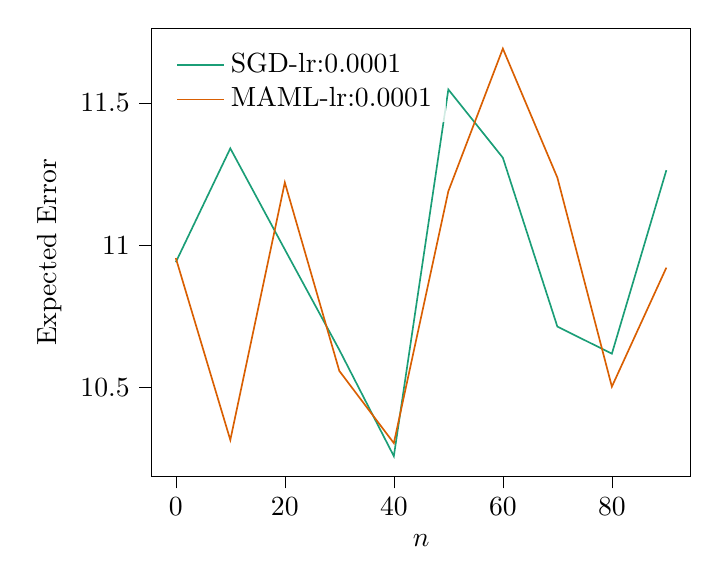
\begin{tikzpicture}

\definecolor{color0}{rgb}{0.105882352941176,0.619607843137255,0.466666666666667}
\definecolor{color1}{rgb}{0.850980392156863,0.372549019607843,0.00784313725490196}

\begin{axis}[
legend cell align={left},
legend style={
  fill opacity=0.8,
  draw opacity=1,
  text opacity=1,
  at={(0.03,0.97)},
  anchor=north west,
  draw=none
},
tick align=outside,
tick pos=left,
x grid style={white!69.0196078431373!black},
xlabel={\(\displaystyle n\)},
xmin=-4.5, xmax=94.5,
xtick style={color=black},
y grid style={white!69.0196078431373!black},
ylabel={Expected Error},
ymin=10.1877620896084, ymax=11.762657966401,
ytick style={color=black}
]
\addplot [semithick, color0]
table {%
0 10.9407338493568
10 11.3405475904374
20 10.9853516591116
30 10.6326820559894
40 10.2593482658262
50 11.547446306611
60 11.307730564726
70 10.7145674141628
80 10.61937007324
90 11.2639238710727
};
\addlegendentry{SGD-lr:0.0001}
\addplot [semithick, color1]
table {%
0 10.9553564532562
10 10.3162068853097
20 11.220765092014
30 10.5587868252572
40 10.3051611970129
50 11.1900065622473
60 11.6910717901832
70 11.2378429971163
80 10.5034800111281
90 10.9217432687916
};
\addlegendentry{MAML-lr:0.0001}
\end{axis}

\end{tikzpicture}
